\section{Reinforcement Learning}


\subsection{What is reinforcement learning}

Reinforcement learning is the study of "learning by interaction". As in the real world, when learning how to act, this is done by trial and error.

\subsection{The Environment/Agent interface}

The problem of learning by trial and error has a natural formulation by the environment/agent interface:

\begin{figure}
    \centering
    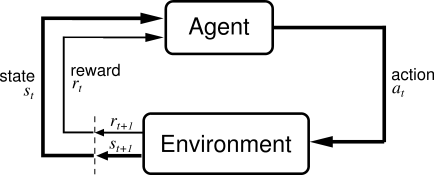
\includegraphics[scale=0.5]{figures/agent_environment_interface.png}
    \caption{Agent/Environment Interface}
    \label{fig:agent_enviroment_interface}
\end{figure}

The problem can be phrased the following way: An agent will over a series of discreet time steps $t=1, 2, \cdots, T$ take an action which will lead to some sort of reward (or in economic terms utility). So for each time step the agent gets information about the environments state $S_t$. The agent can then take an action $A_t$, which prompts the environment to return a reward $R_{t+1}$, and a new state $S_{t+1}$, which restarts the loop until the game terminates. The agents sole purpose is to maximize the cumulative rewards through out the game. It should be noted here that $R_t \in \R$. So the agent is optimizing over a sum of scalars. The representation of the state $S_t$ can be only partially observable in the reinforcment learning formulation. This game will lead to a trajectory of states, actions and rewards that look like:

\begin{equation}
    S_0, A_0, R_1, S_1, A_1, R_2, S_2, A_2, \cdots ,R_{T-1}, S_{T-1}, A_{T-1}, R_{T}
\end{equation}

However more formally certain assumption is necessary to perform any sort of modelling. The most fundamental assumption RL relies on is Markov Decision processes: A Markov decision process (MDP) can be described as:

\begin{equation}\label{eq:mdp1}
    p(s_t, r_t \mid s_{t-1},  a_{t-1}) = p(s_t, r_t \mid s_{t-1},\cdots, s_{0}, a_{t-1}, \cdots, a_{0}) = P(S_t = s_t, R_t = r_t \mid S_{t-1} = s_t, A_{t-1} = a_t)
\end{equation}

Breaking the equation \eqref{eq:mdp1} down we see that the MDP follows a true probability distribution. That is $R_t$ and $S_t$ is well defined probability distributions. More over another very important feature is that the probability distribution of $S_t$ and $R_t$ only depends on the last state and action. This turns out to be a very important assumptions to do any sort modelling. This implies that the state $s_t$ contains all relevant information about the past, which is what makes the problem a \textit{Markov} Decision Process. This condition/assumption yields certain important features. First, it implies that size of the probability distribution would not grow linearly as more and more states and actions was represented for the agent. Yielding the computations more and more expensive. Second thing which is important is, that allows for backward induction and dynamic programming (a topic which will be discussed later). Lastly this implies than when we model the system we must ensure that the state is represents all relevant information about the past.

From the equation \eqref{eq:mdp1} multiple statements can be derived, but most importantly one can derive, the expected rewards, which is what we is what the agent want to maximize:

\begin{equation}
    \E[R_t \mid A_{t-1} = a_{t-1}, S_{t-1} = {s_{t-1}}] = \int_{r_t} \int_{s_t} p(r_t, s_t \mid r_{t-1} s_{t-1}) d s_t d r_t 
\end{equation}

As mentioned in the start the agents goal is to maximize the cumulative rewards. This can be described as in equation:

\begin{equation}\label{eq:cum_rewards}
   G_t = R_{t+1}, R_{t+2}, R_{t+3}, \cdots R_{T}
\end{equation}

In general however the above formulation can be problematic with continuing tasks. That is if $T \rightarrow \infty$. Therefore discounting of rewards is usually implemented. Which have the nice economic implications, that agents in the real world tend to be impatient, and therefore more realistically real human agents:

\begin{equation}
    G_t = R_{t+1} + \gamma R_{t+2} + \gamma^2 R_{t+3} + \cdots = \sum_{k=0}^{T - t} \gamma^k R_{t+k+1}
\end{equation}

with $\gamma$ being the discount rate, yielding a geometric series, that is known to converge, if $R_k$ is bounded.

\subsection{Value function, Q-function, Policy function and the Bellman Equation}

To navigate in the environment usually a couple of things is considered: First the value-function:

\begin{equation}\label{eq:value_function1}
    v_{t}^{\pi}(s_t) = \E_t [G_t \mid S_t = s_t] = \E_t \lsp \sum_{k=0}^{T - t} \gamma^k R_{t+k+1} \bigg\vert S_t = s_t \rsp 
\end{equation}

Where it's implied in this formulation that the agent is following some policy $\pi$. A couple of things to note about \eqref{eq:value_function1}: Since the expectation is taken over a sum this is the same to take the sum over the expectations, yielding it possible to calculate the individual expected returns from following a policy, and using those to calculate the value function. Another formulation that lies close to the value-function is the Q-function which will be explored in this paper:

\begin{equation}
    q_t^{\pi} (s_t, a_t) = \E_t [G_t \mid S_t = s_t, A_t = a_t ] = \E_t \lsp \sum_{k=0}^{T - t} \gamma^k R_{t+k+1} \bigg\vert S_t = s_t, A_t = a_t\rsp 
\end{equation}

which only differ from the value function by also conditioning on the action, and not only the state. The value function and the Q-function shares the property that it maps the expected value of an state (or state action pair) to a scalar vale, where this value represent the cumulative, discounted rewards of following a certain policy. This has the nice property of allowing the agent to choose an action which maps to the highest expected value.

A policy function is a how the agent chooses its actions:

\begin{equation}
    \pi_t : \statespace \mapsto \actionspace 
\end{equation}

Some of the methods explored in this paper works by directly estimating the policy function, where as other works by estimating the value function or Q-function using these to find the correct optimal policy.

Using the expression of the value function we can now express the Bellman equation:

\begin{equation}
    v^{\pi}_{t} (s_t) = \E_t [G_t \mid S_t] = \E_t  \lsp R_{t+1} + \gamma G_{t+1} \mid S_t \rsp = \E_t \lsp R_{t+1} + \gamma v_{t+1}^{\pi}(s_{t+1}) \rsp
\end{equation}

A couple of things to note about the bellman equation: First and foremost one should consider that $\E [v_{t+1}^\pi(s_{t+1})]$ does not imply $v_{t+1}^{\pi}(\E[s_{t+1}])$, which has the consequence of considerable computational markup when solving a model using the Bellman Equation. Furthermore.

\subsection{Relationship to Dynamic Programming}\label{sec:dynamic_programming}

\textbf{BOOTSTRAP SKAL INTRODUCERES}

Dynamic programming, invented by Richard Bellman, and allows for a way to find the optimal policy $\pi^{*}$ and the associated value function $v^{\pi^{*}}$ when following the optimal policy. To do dynamic programming, certain things are necessary. First the size of the statespace should be limited. That is due to the fact, that number of computations will increase exponentially with the number of states. Secondly it also requires that the entire MDP is known. So partially observable models f.x. cannot be used. In general it can be said that dynamic programming (and also reinforcement learning) is to use the value function to structure the search for good policies  (XXX Sutton and barto). It's clear that if we have the optimal value function, we also have the optimal policy:

\begin{equation}
    v_t^{*}(s_t) = \underset{a_t}{\max} \lsp \E \lsp R_{t+1} + \gamma v^{*}_{t+1}(s_{t+1}) \mid S_t = s_t, A_t = a_t\rsp \rsp
\end{equation}

Dynamic programming problems can be solved by two different approaches: value function iteration and policy function iteration.

Policy function iteration consists of two steps: 1) an evaluation step. Which calculates the value of a policy, and 2) a policy improvement step.
Step 1 can be considered a prediction step, that by following a given policy calculates the associated value function for said policy. This is done by sweeping through the state space calculating the expected value of the state following the policy. This process continues until the algorithm has converged, where converged implies that the difference between the previous estimation of the value function and the current estimation of the value function, only differs below some threshold. The second step, policy improvement, follows the logic. Assume that the policy just used for the evaluation step is optimal. Then there should be no other strategy that would yield a higher value-function for all possible states. Now this can be written more formally as:

\begin{equation}
    \pi^*_t (s_t) \geq \tilde{\pi}(s_t)\qquad \forall s_t \in \statespace
\end{equation}

where $\tilde{\pi}$ is any arbitrary strategy. This also implies that if we at any point in the state space can find a policy that yields a higher value function than the current, then we should switch strategy. Which have now yielded a better strategy! If the during the sweep through state space, searching for better policies, a new policy is found. The process goes back to a policy evaluation step. This goes on until that there can be found no better policy than currently being employed. A graphical the process can be considered as shown in equation \eqref{eq:policyevaluation} where $\overset{\textbf{E}}{\longrightarrow}$ denotes a policy evaluation and $\overset{\textbf{I}}{\longrightarrow}$ denotes policy improvement:

\begin{equation}
    \label{eq:policyevaluation}
    \pi^0 \overset{\textbf{E}}{\longrightarrow}
    v^{\pi^0} \overset{\textbf{I}}{\longrightarrow} \pi^1 \overset{\textbf{E}}{\longrightarrow} v^{\pi^1} \overset{\textbf{I}}{\longrightarrow} \cdots \overset{\textbf{I}}{\longrightarrow} \pi^* \overset{\textbf{E}}{\longrightarrow} v^{\pi^*}
\end{equation}

The second approach value function computes a max over the value function implying only a single sweep through the state space in iteration of the loop, yielding it a much faster approach for solving the model. Value function iteration can be considered using the Bellman equation as an update rule. (Barto and Sutton XXX). The algorithm for value function iteration is described below:

\begin{algorithm}[H]
\SetAlgoLined
\KwResult{Yielding $\pi^*, v^*$}
 Algorithm parameter $\theta > 0$ determining accuracy of estimation\;
 Initialize $V(s)\quad \forall s \in \statespace$ except $V(terminal) = 0$\;
 \While{$\Delta > \theta$}{
    $\Delta \la 0$ \; 
    \ForEach{$s \in \statespace$}{
        $v \la V(s)$ \;
        $V(s) \la \underset{a}{\max} \E [R_{t+1}  + \gamma V(s') \mid A_t = a, S_t = s] $ \;
        $\Delta \la \max (\Delta, \mid  v - V(s) \mid )$
    }
 }
 \caption{Value Function Iteration}
\end{algorithm}

 So for each step sweep through the loop a single sweep through the state space is performed finding which action yields the highest associated value for a given state. Finally when the sweep is completed the associated policy evaluation can be done. Finding the value function. Again this algorithm terminates when the difference between the value function of the last sweep and the current value function is below some threshold.
 
 In economics very often a dynamic model will be solved using value function iteration but with the addition of using backwards induction. How is this possible. Just as the model presented in this paper. The model assumes an agent acting over $T$ time steps, terminating when the agent reaches a certain age. So in a sense the agent moves in a deterministic fashion towards the termination of the environment. This implies that one can solve such a model by only doing a single sweep through the state space! What will be done is that at the terminal period the agent will optimize his value function. Now using this value associated with the terminating period, the agent can consider his actions in $T-1$. Remembering that we can use the Bellman equation as an update step we can write:
 
 \begin{equation}
     V_{T-1}(s_{T-1}) = \underset{a_{T-1}}{\max}\E [R_{t+1} + \gamma V_T (s_T)]
 \end{equation}
 
 In other words, we can model all possible states that the agent can encounter in each time step of the model, making it possible to find the optimal value function $v^{\pi^*}$ and policy function $\pi^{*}$ by simple sweep through the state space using a combination of dynamic programming and backwards induction. The implementation of Value function iteration in this paper will be explored in a later section.
 
 \subsection{Overview of other Reinforcement learning techniques}.
 
Later in this paper I present three different reinforcement learning methods. Here i present some basic information that makes the reader able to digest the material presented. First it's important to address why not only use dynamic programming. Dynamic programming requires that a perfect model of the environment is accessible. This is due to the fact, that when calculating the expected value function for each action, the probability distribution of the reward and the next state, needs to formulated in an explicit form. The other techniques presented here does not have the same requirement. Secondly DP methods require that state space cannot be to large. The implementations presented later does not have the same requirements, allowing for approximating the value function and/or the policy function. Below i explain two different methods of learning \textit{Monte Carlo Methods} and \textit{Temporal Difference Learning} these being the two foundations of the reinforcement learning methods presented later.

\subsubsection{Monte Carlo Methods}

Before delving into MC-methods it is appropriate to introduce some more nomenclature: when talking about an \textit{episode} it should be understood as an agent moving through the environment from start to termination. When talking about a \textit{step} it should be understood as going from one state to the next in the environment. The best way to get a sense of Monte Carlo methods is to present the algorithm:

\begin{algorithm}[H]
\SetAlgoLined
\KwResult{Yielding $v^{\pi}$}
 Input: policy $\pi$ to be evaluated\;
 $Returns(s) \la$ an empty list $s \in \statespace$\; 
 \While{Forever}{
    Generate an episode: $S_0, A_0, R_1, S_1, A_1, \cdots S_{T-1}, A_{t-1}, R_T$\; 
    $G \la 0$ \;
    \ForEach{step in episode, $t = \{T -1 , T-2 , \cdots, 0\}$}{
        $G \la \gamma G + R_{t+1}$\;
        \If{$S_t \notin \{S_{t-1}, S_{t-2}, \cdots S_0 \}$}{
            Append $G$ to $Returns(S_t)$ \;
            $V(S_t) \la average(Returns(S_t))$ \;
        }
    }
 }
 \caption{First-Visit MC prediction, for estimating $v^{\pi}$}
 \label{alg:mcfirstvisit}
\end{algorithm}

Algorithm \ref{alg:mcfirstvisit} shows how the general concept of estimating the value function for given policy. Things to be noted: First and foremost the algorithm presented above is made to a tabular case, i.e discrete state space. This will be dealt with in the algorithm presented later in this paper. Second it is assumed that the policy stays constant. That is, the policy does not update as more and more episodes are experience, which defeats the purpose of learning how to interact with the environment. Addressing the latter part usually the policy is updated, and the you could discard the old experience. However another possibility is to accept the non stationarity of the data collected, and update the policy using the data from a previous policy, hoping that with time the algorithm will converge.

Consider now how to do Monte Carlo Control, i.e. approximating the optimal policy. Just as with policy iteration the pattern followed is:

\begin{equation}
    \label{eq:montecarlocontrol}
    \pi^0 \overset{\textbf{E}}{\longrightarrow}
    q^{\pi^0} \overset{\textbf{I}}{\longrightarrow} \pi^1 \overset{\textbf{E}}{\longrightarrow} q^{\pi^1} \overset{\textbf{I}}{\longrightarrow} \cdots \overset{\textbf{I}}{\longrightarrow} \pi^* \overset{\textbf{E}}{\longrightarrow} q^{\pi^*}
\end{equation}

Just with the caveat that instead of considering the value function, the Q-function (state-action pair) is used for policy evaluation. Policy improvement is done by making the policy greedy with respect to the current estimated Q-function (XXX Barto and sutton). Since the Q-function instead of the value function is used, no model us needed to construct a greedy policy (XXX barto and Sutton). The greedy policy is the one that for each $s \in \statespace$ deterministically chooses an action with maximal action-value:

\begin{equation}
    \pi(s) = \underset{a}{\argmax}  q( s, a )
\end{equation}

Now this algorithm is made under the assumption of \textit{exploring starts} and under the assumption of \textit{infinite epsiodes}. The assumption of inifinte episodes is to ensure convergence, and in practice the algorithm is usually run until the algorithm has converged by some high number of episodes. The more problematic assumption is that of exploring starts. This is due to the fact, that in reality we would not assume that there is a uniform distribution of starting in all states $s \in \statespace$, and proceed the episode from that starting point. This is an essential assumption, because otherwise, one could not know the value function of unexplored states without visiting them. This leads to the concept of on-policy control. On policy control is most often implemented using an $\epsilon$-greedy strategy. The implication is that $P(A=a \mid S=s, q^{\pi}) > 0, \forall a \in \actionspace, s \in \statespace$. Where the non optimal action is choosen by drawing from an uniform distribution over all actions with probability $\epsilon$. Off-policy control works by having two different policies one which works by doing the optimal action (target policy $\pi$), and a second policy that moves to investigate the state space (behavior policy $b$). Using the experience from these two policies importance sampling can be used to estimate the value function! It's required that the behavior policy has a non zero probability to any action for any state.

\subsubsection{Temporal Difference Learning}

Temporal Difference (TD) learning is a combination of ideas taken from Dynamic Programming and Monte Carlo Methods. It takes from Monte Carlo methods, that you do not need a perfect model of the environment. It takes from Dynamic Programming the bootstrapping, i.e. it uses learned estimates to update, without needing the final outcome. Just as Monte Carlo methods, Temporal difference methods has a prediction and control element. 

TD prediction can be summarized in the equation:

\begin{equation}
    V(S_t) \leftarrow V(S_t) + \alpha \lsp R_{t+1} + \gamma V(S_{t+1}) - V(S_t) \rsp
\end{equation}

The equation states that $V(S_t)$ should be updated according to the return in a given period + the value function of the next period $V(S_{t+1})$. This method is called TD(0), since it only uses 1 step to update the value function. In essence TD methods learn a guess from a guess. This allows for not having a complete model of the environment (of rewards and next-state probability distributions). Compared to MC methods the TD learning can learn at each step - update it's estimate at each point in time. It is also proven, that for any policy $\pi$ kept fixed, then a TD(0) algorithm will converge to $v^{\pi}$ (XXX Barto and Sutton). Even though, an open mathematical question, in practice it is found that TD methods converge faster than MC methods (XXX Barto and Sutton).

Control with temporal difference learning, can also be separated into on-policy control and off-policy control. The most used on-policy control for TD methods is called SARSA (state, action, reward, state, action). Just as with MC methods a need to trade off exploitation and exploration is present. The agent want to see new parts of the state space (exploration), but should also use exploit what is assumed to be the optimal choice given the value function associated with the current value function. In this case instead of using the value function instead, consider the case of using the state-action pair function $Q(S_t, A_t)$, yielding the update rule:

\begin{equation}
    Q(S_t, A_t) \leftarrow Q(S_t, A_t) + \alpha \lsp R_{t+1} + \gamma Q(S_{t+1}, A_{t+1}) - Q(S_t, A_t) \rsp
\end{equation}

This update is made after each step in a non-terminal state of the environment. As in on-policy methods $q^{\pi}$ is estimated for the policy $\pi$ whilst at the same time greedy updating $\pi$ with respect to $q^{pi}$. Exploration can again be done using an epsilon greedy approach.

Off-policy control can be done by using Q-learning. Q-learning has the slight twist on update the rule for SARSA that:

\begin{equation}
    Q(S_t, A_t) \leftarrow Q(S_t, A_t) + \alpha \lsp R_{t+1} + \gamma \underset{a}{\max} Q(S_{t + 1}, a) - Q(S_t, A-t) \rsp 
\end{equation}

Actions is still chosen by an $\epsilon$-greedy policy, the difference here being the updating rule presenting a different policy than the actual policy, since we assume that we greedily chooses the action in time $t+1$ conditional on the state. Q-learning and double Q-learning will be explored in depth later when describing the algorithms used in this paper.

\subsection{Landmarks}

Finally, before moving a brief overview of environments/games where reinforcement learning have been instrumental. The first big success of reinforcement learning was made by Tesauro in 1992 creating an agent of learning to play backgammon trough self play. Using an artificial neural network to approximate the value function, and using a temporal difference algorithm, the algorithm was capable of playing expert level backgammon. In 2011 the IBM Watson algorithm won in jeopardy using the same methods as Tesauro for his backgammon agent. In 2013 the company DeepMind (now acquired by google), showed that it was possible for a reinforcement learning algorithm to learn to play video games. Here an important feat was, that it was fed the raw image input and used an artificial neural network to transform this image into an representation of the state space allowing for learning how to navigate in the environment. in 2016 DeepMind created AlphaGo and a year later AlphaGo Zero, which learned to master the game of Go. This was assumed in a long time to be a hard problem for learning algorithm due to its very large state and action space. The first iteration used expert players to learn the game, while the AlphaGo zero used only selfplay. These examples show that the feasibility of these algorithms to learn to navigate in complicated environments, might leave a way for high dimensional dynamic economic models to be solved using reinforcement learning methods.